\chapter{Tool Analysis: Existing Approaches to Container Energy Consumption} % Main chapter title
\label{Chapter4}

\section{Overview of Tool Landscape}
            KEPLER, Scaphandre, CodeCarbon, PowerAPI, Cloud Carbon Footprint, etc.
\section{Tool Analysis Framework}
        Accuracy, data sources, correlation method, platform support, etc.
\section{Detailed Evaluation of Selected Tools}
        One subchapter per tool:
            4.X KEPLER
            4.X Scaphandr
            ...
\section{Comparison Summary}
        Table of tradeoffs
        Strengths and weaknesses
        Missing features / open gaps



\chapter{Tool Analysis: Existing Approaches to Container Energy Consumption}
\label{chap:tool-analysis}

\section{Introduction}
\label{sec:tool-intro}

\section{Non-Kubernetes Energy Monitoring Tools}
\label{sec:non-k8s-tools}
\subsection{Server-Level Energy Monitoring}
\label{sec:server-tools}
While not directly translatable to container-level energy monitoring, server-level energy consumption is an important aspect of it. Scientific works and tools in this domain generally don't provide the temporal resolution required for container-level energy monitoring.

\subsubsection{Kavanagh and Djemame: Energy Modeling via IPMI and RAPL Calibration}
\label{sec:kavanagh}

\paragraph{Overview and Architecture}
Kavanagh and Djemame\parencite{kavanagh2019rapid} present their findings on combining IPMI and RAPL (interface unspecified) data to estimate server energy consumption, achieving improved accuracy through calibration with an external server-level Watt meter. For calibration, they induce artificial CPU workloads and rely on CPU utilization metrics with 1-minute averaging windows, necessitating extended calibration intervals to obtain stable readings. While the resulting model is tailored to their specific hardware and not generally portable, their work provides valuable insights into the complementary use of IPMI and RAPL. The authors recognize that the respective limitations of these tools (RAPL’s partial scope and IPMI’s low resolution) can be mitigated when used in combination.

\paragraph{Attribution Method and Scope}
Although the model operates at the physical host level, it supports attribution to VMs or applications using CPU-utilization-based proportional allocation. Several allocation rules are proposed, including utilization ratio, adjusted idle sharing, and equal distribution. However, no container-level attribution is attempted, and runtime flexibility is limited due to the static nature of the calibration.

\paragraph{Validation and Limitations}
With their Watt-meter-calibrated model using segmented linear regression, the authors report an average error of just -0.17\%. More relevant to practical application, they also construct a model based solely on IPMI and RAPL(calibrated via Watt meter data) which achieves a reduced error of -5.58\%, compared to -15.75\% without calibration. Limitations of their approach include the need for controlled, synthetic workloads, coarse-grained sensor input, and the assumption of relatively stable system conditions during calibration.

\paragraph{Key Contributions}
\begin{itemize}
    \item \textbf{Hybrid use of IPMI and RAPL is analyzed}, showing that these tools compensate for each other’s limitations. RAPL underestimates total system power, while IPMI captures more components but at lower resolution.
    \item IPMI accuracy is significantly improved through external Watt meter calibration.
    \item The authors provide practical calibration guidelines:
    \begin{itemize}
        \item Use long, static workload plateaus to align with averaging windows and reduce synchronization complexity.
        \item Discard initial and final measurement intervals to avoid transient noise and averaging artifacts.
        \item Ensure calibration workloads exceed the IPMI averaging window to capture valid steady-state values.
    \end{itemize}
\end{itemize}

\paragraph{Relevance to Proposed Architecture}
This work informs the proposed architecture by demonstrating how combining RAPL and IPMI can yield more accurate system-level power estimation. The use of plateau-based calibration and composite data models is especially applicable. However, the lack of container-level granularity, reliance on offline calibration, and limited attribution scope underscore the need for more dynamic, fine-grained, and container-aware approaches in Kubernetes-based environments.

\subsubsection{CodeCarbon}
CodeCarbon\parencite{codecarbon_2024} is a Python package designed to estimate the carbon emissions of a program’s execution. While its implementation is general-purpose, it is primarily aimed at machine learning workloads.

\paragraph{Overview and Architecture}
CodeCarbon estimates a workload’s energy consumption by relying on RAPL \textit{package-domain} CPU metrics via the \texttt{powercap} RAPL file system interface. A fix for the RAPL MSR overflow issue was implemented\parencite{codecarbon_issue_322}. In the absence of RAPL support, it falls back to a simplified model based on the CPU’s Thermal Design Power (TDP), obtained from an internal database, and combines it with CPU load metrics from \texttt{psutil}. For memory, a static power value is assumed based on the number and capacity of installed DIMMs. GPU power consumption is estimated via NVIDIA’s NVML interface. The default measurement interval is 15 seconds, with the authors citing lightweight design as the primary motivation.

The component-level estimations are then aggregated and multiplied by a region-specific net carbon intensity (based on the local electricity grid’s energy mix) to estimate the program’s total CO\textsubscript{2} emissions. CodeCarbon is typically executed as a wrapper around code blocks, scripts, or Python processes.

\paragraph{Limitations}
There is no direct attribution of CPU activity to individual power metrics: CodeCarbon estimates energy use indirectly, based on the number of active cores and average CPU utilization, while making many assumptions that could be prevented. Combined with the relatively long measurement intervals, this results in background system processes also being attributed to the measured Python program. Consequently, CodeCarbon does not contribute directly to the goals of this thesis, which seeks fine-grained, container-level attribution.

However, the tool highlights several interesting secondary considerations. The integration of regional CO\textsubscript{2} intensity data is a valuable extension to conventional energy measurement and is well implemented. Additionally, the Python-based design offers high accessibility and ease of use, which may serve as inspiration for future developer-facing tools.

\subsubsection{AI Power Meter}
\textit{AI Power Meter}\parencite{aipowermeter} is a lightweight Python-based tool designed to monitor the energy consumption of machine learning workloads. It gathers power consumption data for the CPU and RAM via Intel RAPL using the \texttt{powercap} interface, and for the GPU via NVIDIA’s NVML library. While the authors acknowledge that other system components (e.g., storage, network) also contribute to energy usage, these are not currently included and are considered an accepted limitation of the tool.

Unlike more advanced attribution tools, AI Power Meter does not distinguish between individual processes or workloads. Instead, it provides coarse-grained, system-level energy consumption measurements over time. In this respect, its scope is similar to \textit{CodeCarbon}, focusing on ease of use and integration into ML pipelines rather than precise, per-process energy attribution. As such, while not directly applicable to container-level measurement or power attribution, AI Power Meter demonstrates the growing interest in accessible energy monitoring tools within the machine learning community.

\subsection{Process-Level Attribution Tools}
\label{sec:process-tools}
\subsection{Telemetry-Based Estimation Frameworks}
\label{sec:telemetry-tools}

\subsubsection{PowerAPI Ecosystem\parencite{powerapi2024github} (PowerAPI, HWPC, SmartWatts)}
\label{sec:powerApiFramework}

PowerAPI\parencite{fieni2024powerapi} is an open-source middleware toolkit for assembling software-defined power meters that estimate real-time power consumption of software workloads. Developed as a generalized and modular framework, PowerAPI evolved alongside specific implementations such as \textit{SmartWatts}, detailed in section~\ref{sec:smartwatts}. It allows power attribution at multiple granularity levels, including processes, threads, containers, and virtual machines. A distinctive strength of PowerAPI is the continuous self-calibration of its power models, enabling accurate real-time energy estimation under varying workloads and execution conditions. This makes PowerAPI particularly suited to heterogeneous computing infrastructures.

\paragraph{Overview and Architecture}

PowerAPI uses an actor-based model for modularity, enabling easy customization of its internal components with minimal coupling. It supports raw metric acquisition from diverse sensors (e.g., physical meters, processor interfaces, hardware counters, OS counters) and delivers power consumption data through various output channels (including files, network sockets, web interfaces, and visualization tools). As middleware, PowerAPI facilitates assembling power meters "\textit{à la carte}" to accommodate specific user requirements and deployment scenarios.

\paragraph{Core Components}
\begin{itemize}
    \item \textbf{powerapi-core}: Middleware orchestrating real-time/post-mortem interactions between sensors and formulas. It defines the essential interfaces for sensor data ingestion and output channels (e.g., MongoDB, InfluxDB, CSV, socket, Prometheus), and includes built-in capabilities for data preprocessing, postprocessing, and reporting.
    \item \textbf{hwpc-sensor}: A telemetry probe designed to gather low-level hardware performance counters (HWPCs), including instructions, cycles, and RAPL energy metrics. This sensor leverages \textit{perf} and \textit{cgroups-v2}, critical for fine-grained telemetry in containerized environments. It also provides detailed CPU performance state metrics via MSR events (\texttt{TSC}, \texttt{APERF}, \texttt{MPERF}).
    \item \textbf{SmartWatts-formula}\parencite{fieni2020smartwatts}: A power model implementation (in Python) using HWPC data to estimate power consumption dynamically. It employs online linear regression provided by the Python \textit{scikit-learn}\parencite{scikit-learn} library, enabling accurate runtime learning of workload-specific power signatures. SmartWatts is further detailed in section~\ref{sec:smartwatts}.
    \item \textbf{SelfWatts-controller}: Dynamically selects hardware performance counters for software-defined power models, facilitating automatic configuration and unsupervised deployment in heterogeneous infrastructures. Currently, its development has stalled for several years, limiting its practical applicability.
    \item \textbf{pyRAPL}: A convenient Python wrapper around RAPL for CPU, DRAM, and iGPU energy metrics collection, providing easy access to hardware-based power data.
\end{itemize}

\paragraph{Relevance and Integration}
The modular and extensible architecture of PowerAPI positions it as a highly suitable foundation for further research and development of specialized power attribution tools. Researchers can readily extend or adapt its components to address evolving or niche requirements. However, its current implementation does not incorporate certain critical metrics, such as IPMI-based telemetry, which could limit its completeness in some practical deployment scenarios. Nonetheless, PowerAPI represents a significant advancement toward the creation of generalized, plug-and-play power models that operate without extensive manual calibration. This emphasis on practical deployability and general applicability highlights a key strength of the project and sets a clear direction for future research and development efforts in the domain of software-defined energy monitoring.





\section{Code-Level and Adjacent Energy Profiling Tools}
\label{sec:code-tools}
\subsection{Compiler and Instruction-Level Estimation}
\label{sec:compiler-tools}
\subsection{Runtime Profilers and System Tuning Tools}
\label{sec:runtime-tools}
\subsection{Machine Learning-Based Estimators}
\label{sec:ml-estimators}

\section{Container-Focused Energy Attribution Tools}
\label{sec:container-tools}

\subsection{Kepler}
\label{sec:kepler}
\subsubsection{Overview and Goals}
\label{sec:kepler-overview}
\subsubsection{Architecture and Metric Sources}
\label{sec:kepler-architecture}
\subsubsection{Attribution Model and Output}
\label{sec:kepler-attribution}
\subsubsection{Validation and Research Context}
\label{sec:kepler-validation}
\subsubsection{Limitations and Open Issues}
\label{sec:kepler-limitations}

% \subsection{Scaphandre}
% \label{sec:scaphandre}

% \subsubsection{Overview and Goals}
% \label{sec:scaphandre-overview}

% Scaphandre\parencite{scaphandre_github} is an energy monitoring agent designed to expose power consumption metrics at a fine granularity, particularly for containerized and virtualized environments. Its name (derived from the French word for diving suit) reflects the tool’s aim to provide deep insight into system-level energy consumption.

% Scaphandre aims to attribute energy usage to individual processes, containers, or pods. Scaphandre offers multiple deployment models: It can be deployed directly to a host (and measure qemu/kvm virtual machines), or in a container and measure the power consumption of the bare metal host, provided that \texttt{/sys/class/powercap} and \texttt{/proc} directories are exposed as volumes. Most importantly in the context of this thesis, it can be directly installed on kubernetes via Helm chart (along with \textit{Prometheus} and \textit{Grafana}) and measure Kubernetes nodes and containers, increasing convenience and ease-of-use.

% \subsubsection{Architecture and Metric Sources}
% \label{sec:scaphandre-architecture}
% Scaphandre is written in Rust. Its core architecture is modular and extensible, consisting of two main components: \textit{sensors} and \textit{exporters}. Sensors are responsible for gathering energy-related data from the host system, while exporters format and expose this data to external systems. This design allows Scaphandre to integrate into cloud-native environments, supporting observability stacks and automation tools.

% \paragraph{\textit{Sensors}}
% Scaphandre's \textit{Sensors} subsystem is meant to get utilization and power consumption metrics of the host, and make them available to the exporter(s). An abstration layer (implemented in the \texttt{/sensors/mod.rs}-file) manages the system typology (including sensors, domains, processes and CPU) and Record generation. 

% Scaphandre’s \texttt{PowercapRAPLSensor} (implemented in the \texttt{powercap/textunderscorerapl.rs}-file) builds a power topology by reading Intel RAPL data from the \texttt{/sys/class/powercap} interface. By default, it identifies all available domains (for all available sockets) using directories that match the pattern \texttt{intel-rapl:<socket>:<domain>}, each containing the domain name and its cumulative energy in microjoules. If no domain-level directories are found, Scaphandre triggers a fallback, omitting subdomain breakdowns. In this case, it reads only the socket-level file: \texttt{/sys/class/powercap/intel-rapl:<socket>/energy/textunderscoreuj}. This file corresponds to the \texttt{package} (PKG) domain, which represents the total energy for the CPU socket. While PKG is technically a RAPL domain, it also serves as the root of the domain hierarchy.

% In addition to the Powercap RAPL sensor implementation, a Windows-only RAPL sensor is also implemented using direct MRS read-operations of Intel or AMD-specific MSRs.

% System utilization metrics are read by the sensors implemented in \texttt{utils.rs}, using Rust’s \texttt{sysinfo} and \texttt{procfs} crates. These libraries extract information from virtual filesystems such as \texttt{/proc}, \texttt{/sys}, and \texttt{/dev}. When container support is enabled, cgroups are also read—but solely for the purpose of mapping processes to containers. The collected metrics are stored in a custom data structure along with timestamps, while cgroup metadata is attached to processes as supplementary labels.

\subsection{Scaphandre}
\label{sec:scaphandre}

\subsubsection{Overview and Goals}
\label{sec:scaphandre-overview}

Scaphandre\parencite{scaphandre_github} is an energy monitoring agent designed to expose power consumption metrics at fine granularity, particularly in containerized and virtualized environments. Its name, derived from the French word for "diving suit" reflects its goal of providing deep insights into system-level energy consumption.

Scaphandre aims to attribute energy usage to individual processes, containers, or pods. It supports multiple deployment models: it can be installed directly on a physical host (where it can also monitor qemu/KVM-based virtual machines) or deployed in a container, measuring the energy usage of the host system, provided that the \texttt{/sys/class/powercap} and \texttt{/proc} directories are mounted as volumes. Most relevant to this thesis, Scaphandre can also be deployed on a Kubernetes cluster via a Helm chart, optionally alongside \textit{Prometheus} and \textit{Grafana}, allowing for convenient monitoring of Kubernetes nodes and containers.

\subsubsection{Architecture and Metric Sources}
\label{sec:scaphandre-architecture}

Scaphandre is written in Rust and features a modular, extensible architecture built around two core components: \textit{sensors} and \textit{exporters}. Sensors gather energy-related data from the host system, while exporters format and expose this data to external systems. This design allows seamless integration into cloud-native observability stacks and automation pipelines.

\paragraph{\textit{Sensors}}

Scaphandre’s \textit{Sensors} subsystem collects utilization and energy consumption metrics from the host system and makes them available to exporters. An abstraction layer, implemented in \texttt{sensors/mod.rs}, manages system topology (tracking sensors, CPU sockets, RAPL domains, and processes) and manages the generation of metric records.

The default Linux implementation, \texttt{PowercapRAPLSensor} (located in \texttt{powercap\_rapl.rs}), constructs a power topology by reading Intel RAPL data from the \texttt{/sys/class/powercap} interface. By default, it identifies all available domains (across all sockets) by matching directories with the pattern \texttt{intel-rapl:<socket>:<domain>}, each containing a domain name and an \texttt{energy\_uj} file reporting cumulative energy in microjoules. If no domain-level directories are found, Scaphandre triggers a fallback mechanism that omits subdomain detail and instead reads from the socket-level file, if available. This file represents the \texttt{package} (PKG) domain, which aggregates the energy consumption of the entire CPU socket. While PKG is a standalone RAPL domain, it also serves as the root of the domain hierarchy. Notably, Scaphandre does not currently handle overflow in the \texttt{energy\_uj} counter, a known limitation that has not yet been resolved despite user-reported inaccuracies~\cite{scaphandre_issue280}.

In addition to the Powercap-based sensor, a Windows-only sensor is available that reads energy consumption directly from Intel or AMD-specific Model-Specific Registers (MSRs).

System utilization metrics are collected by helper functions implemented in \texttt{utils.rs}, which rely on Rust’s \texttt{sysinfo} and \texttt{procfs} crates. These libraries extract data from virtual filesystems such as \texttt{/proc}, \texttt{/sys}, and \texttt{/dev}. When container support is enabled, cgroups are also read—but solely to map processes to containers. The collected metrics are stored in a custom data structure along with timestamps, while cgroup information is attached to each process as additional metadata labels. Apart from metrics of processes, CPU and memory, disk read/write operations are also collected.

\paragraph{\textit{Exporters}}
\textit{Exporters} are responsible for collecting metrics from sensors, storing them temporarily, and exporting them to external systems. Crucially, they also perform the attribution of energy and system metrics to specific scopes, which is discussed in detail in the following section. Similar to the sensor subsystem, Scaphandre uses an abstraction layer (implemented in \texttt{exporters/mod.rs}) to manage common exporter logic such as metric preparation and attribution. Individual exporters are implemented as pluggable modules and operate on a shared core. The \texttt{MetricGenerator} plays a central role by consolidating and attributing metrics across all scopes: the Scaphandre agent itself, the host, CPU sockets, RAPL domains, system-wide statistics, and individual processes.

The modular exporter architecture enables easy implementation of new output formats, and Scaphandre explicitly encourages developers to implement custom exporters if needed. Currently, exporters exist for \textit{Prometheus}, \textit{Stdout}, \textit{JSON}, and \textit{QEMU}, among others.

The \textit{QEMU} exporter is particularly notable. It is designed for use on QEMU/KVM hypervisors and allows energy metrics to be exposed to virtual machines (VMs) in the same way that the \texttt{powercap} kernel module does on bare-metal systems. Specifically, the QEMU exporter writes VM-specific energy metrics to a virtual file system. Inside the VM, a second Scaphandre instance (using the \texttt{PowercapRAPL} sensor with the \texttt{--vm} flag) can read these files, as if they were native energy interfaces. This mechanism mimics a bare-metal powercap environment, allowing software running in the VM to access energy data without direct access to RAPL or hardware sensors. This architecture is especially useful for breaking the opacity of power monitoring in virtualized environments, where such metrics are usually unavailable. If adopted by cloud providers, this could significantly improve visibility into energy consumption within public cloud VMs, supporting energy-aware software design even in virtualized infrastructures.

\subsubsection{Attribution Model}
\label{sec:scaphandre-attribution}

















\subsubsection{Validation and Research Context}
\label{sec:scaphandre-validation}
\subsubsection{Limitations and Open Issues}
\label{sec:scaphandre-limitations}
The developers acknowledge the lack of appropriate RAPL documentation, especially the definition of the \texttt{PSys} domain (which they assume to contain the power specifications of the entire SoC). They also state that their experiments do not clearly indicate whether the \texttt{DRAM} domain is contained in the \texttt{PKG} domain, or outside of it.


\subsection{SmartWatts}


\label{sec:smartwatts}
\subsubsection{Overview and Goals}
\label{sec:smartwatts-overview}
The PowerAPI-implementation \textit{SmartWatts}\parencite{fieni2020smartwatts} is a software-defined, self-calibrating power 'formula' designed for estimating power consumption of containers, processes, and VMs. It aims to address the shortcomings of static power models by using online model adaptation (sequential learning) and runtime performance counters. Unlike many academic models that require manual calibration or architecture-specific training, SmartWatts adapts automatically to the host system and workload.
\subsubsection{Architecture and Metric Sources}
\label{sec:smartwatts-architecture}
SmartWatts is written in Pyhton. Understanding the architecture of SmartWatts and its differences from other energy monitoring tools is crucial. Using HWPC, RAPL, and CPU process metrics, SmartWatts collects performance data. At runtime, it uses power models based on cgroups and perf events alone to estimate, for each resource $\text{res} \in \{\text{CPU}, \text{DRAM}\}$, the host power consumption $\hat{p}_{\text{res}}$ and the power consumption $\hat{p}_{\text{res}}(c)$ for all containers. SmartWatts uses $\hat{p}_{\text{res}}$ to continuously assess the accuracy of the managed power models $M_{\text{res}, f}$ to ensure that estimated power consumption does not diverge from the RAPL baseline measurement $p_{\text{res}}^{\text{rapl}}$. When the estimation diverges beyond a configurable threshold $\epsilon_{\text{res}}$, SmartWatts triggers a new online calibration process for the model. When the machine is at rest (e.g., after a reboot), this method is also used to isolate the static energy consumption. A simple architecture can be seen in Figure~\ref{fig:smartwatts_architecture}.

In practical terms, SmartWatts implements a server-side pwoermeter (referred to as \textit{power meter}) that consumes input samples and produces power estimations accordingly. The power meter is responsible for power modelling, power estimation and model calibration. In addition, a client-side sensor (referred to as \textit{sensor}) is deployed as a lightweight daemon on all cluster nodes. The sensor is responsible static power isolation, event selection, cgroups and event monitoring. This separation allows for heterogeneous cluster nodes.

\begin{figure}[ht]
    \centering
    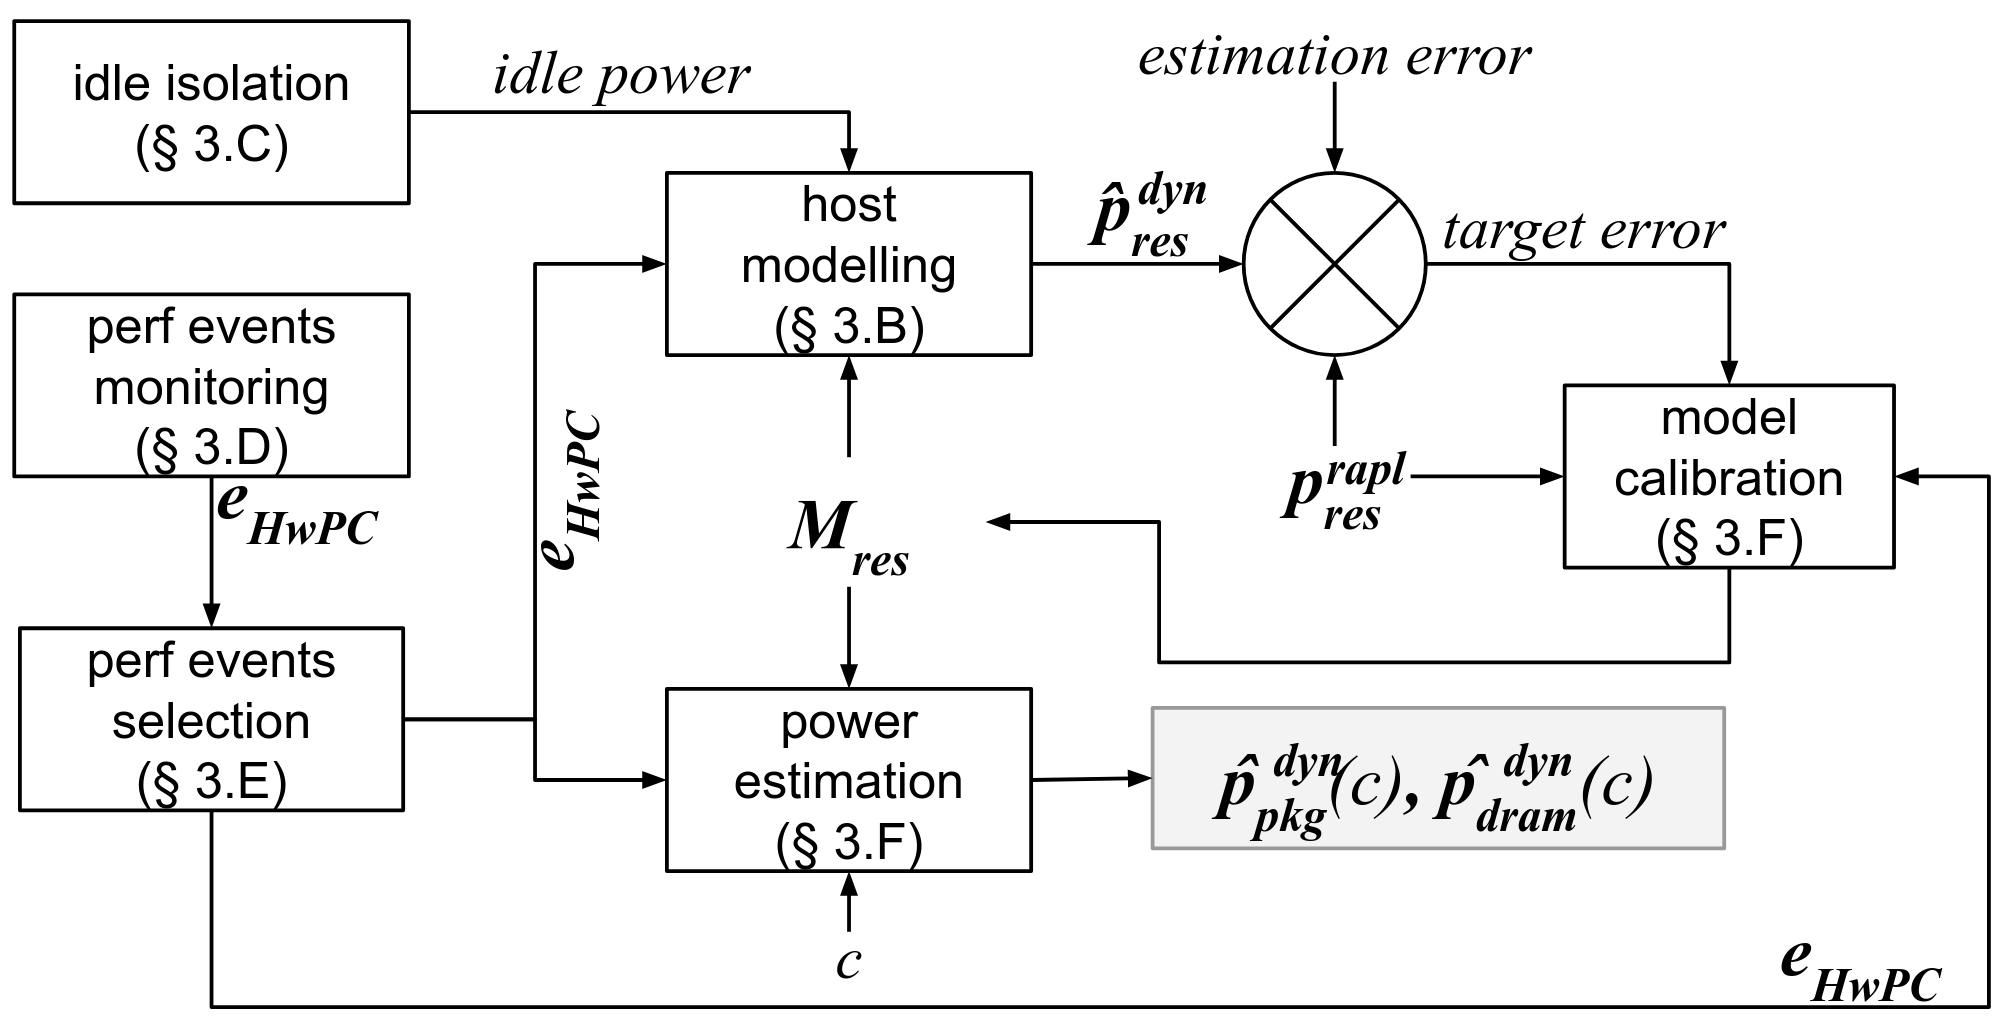
\includegraphics[width=0.7\textwidth]{Figures/smartwatts_architecture.png}
    \caption[SmartWatts architecture]{SmartWatts Architecture}
    \label{fig:smartwatts_architecture}
\end{figure}
\subsubsection{Attribution Model}
\label{sec:smartwatts-attribution}
As discussed in the previous subsection, the SmartWatts attribution model does not use RAPL metrics, opting only for process metrics. SmartWatts separates host energy consumption into static and dynamic power consumption:
\begin{equation}
    p_{res}^{rapl} = p_{res}^{static} + p_{res}^{dynamic}
\end{equation}

\textbf{Static power} is estimated by periodically logging RAPL package and DRAM power consumption. The $median$ value and the $interquartile range$ (IRQ) are gathered from teh measurements to define the static host power consumption as 
\begin{equation}
    p_{res}^{static} := median_{res} - 1.5 \cdot IRQ_{res}
\end{equation}
This approach is meant to filter out RAPL outliers.

\textbf{Dynamic power} is estimated by correlating the CPU frequency $f$ and the raw metrics reported by HWCP:
\begin{equation}
    \exists f \in F, \hat{p}_{res}^{dyn} = M_{res}^{f} \cdot E_{res}^{f}
\end{equation}
where $E_{res}^{f}$ denotes all \textit{events}. The model $M_{res}^{f}$ is build from \textit{elastic net} regression applied on the last $k$ samples. To ensure that all container power consumptions are linear with regards to global power consumption, positive inference coefficients are enforced, and the intercept (or \textit{bias term} is within the range $[0, TDP]$.

\textbf{HWPC metrics} are dynamically chosen based on the list of available events exposed by the host's \textit{Performance Monitoring Units} (PMU), essentially creating a custom model based on available metrics. Not all available metrics are used, and statistical analysis (Pearson coefficient) is used to determining worthy candidates.

\textbf{Container power consumption} is estimated by applying the inferred power model $M_{res}^{f}$ at the scale of the container's events $E_{res}^{f}(c)$, as seen in formula~\ref{for:smartwatts_container_events}. In formula~\ref{for:smartwatts_container_intercept}, the intercept $i$ is distributed proportionally to the dynamic part of the consumption of $c$.
\begin{equation}
\label{for:smartwatts_container_events}
    \exists f \in F, \forall c \in C, \hat{p}_{res}^{dyn}(c) = M_{res}^{f} \cdot E_{res}^{f}(c)
\end{equation}
\begin{equation}
\label{for:smartwatts_container_intercept}
    \forall c \in C, \tilde{p}_{res}^{dyn}(c) = \hat{p}_{res}^{dyn}(c) - i \cdot (1-\frac{\hat{p}_{res}^{dyn}(c) -i}{\hat{p}_{res}^{dyn} -i})
\end{equation}

In theory, one can expect $\hat{p}_{res}^{dyn} \overset{!}{=} {p}_{res}^{dyn}$ if the model perfectly estimates the dynamic power consumption, but in practice, an error $\epsilon_{res} = \left| {p}_{res}^{dyn} - \hat{p}_{res}^{dyn} \right|$. Therefore, container power consumption is capped at
\begin{equation}
    \forall c \in C, \left\lceil \tilde{p}_{res}^{dyn}(c) \right\rceil = \frac{{p}_{res}^{dyn} \cdot \tilde{p}_{res}^{dyn}(c)}{\hat{p}_{res}^{dyn}}
\end{equation}
This approach also allows to calculate a confidence intercal of the power consumption of containers by scaling down the observed global error:
\begin{equation}
    \forall c \in C, \epsilon_{res}(c) = \frac{\tilde{p}_{res}^{dyn}(c)}{\hat{p}_{res}^{dyn}} \cdot \epsilon_{res}
\end{equation}

In order improve estimation accuracy, the following configurable parameters are used:
\begin{itemize}
    \item CPU-TDP in Watt (default: 125)
    \item CPU base clock in MHz (default: 100)
    \item CPU base frequency in MHz (default: 2100)
    \item CPU and DRAM error threshold in Watt (default: 2)
    \item Minimum of samples required before trying to learn a power model (default: 10)
    \item Size of the history window used ot keep samples from (default: 60)
    \item Measurement frequency in milliseconds (default: 1000)
\end{itemize}
\subsubsection{Validation and Research Context}
\label{sec:smartwatts-validation}
With RAPL being used as ground truth for dynamic power estimation model recalibration, it is important to note that the SmartWatts validation is focused on the model accuracy when compared to RAPL values instead of values obtained by an external source of power data. The SmartWatts validation focused on the quality of power estimation in sequential and parallel workloads, the accuracy and sstability of power models and the overhead of the \textit{sensor} component. Standard benchmarks like Stress-NG and NAS parallel Benchmarks were chosen. 

While there is no advanced statistical analysis, the validation shows that, for a error threshold for CPU and DRAM of 5 and 1 Watt respectively, power consumption can be reliably estimated with less than 3 Watts and 0.5 Watts, respectively. The only case where the error grows beyond the threshold is at the CPU idle frequency. The model stability is shown to significantly improve when lower recalibration frequencies are used. SmartWatts succeeds to reuse a give power model for up to 594 estimations, depending on frequency. The monitoring overhead is observed to be at 0.333 Watts for the PKG domain and 0.030 Watts for the DRAM domain on average, at a measurement frequency of 2 Hz. The authors consider this overhead negligable.
\subsubsection{Limitations and Open Issues}
\label{sec:smartwatts-limitations}
SmartWatts offers a compelling solution for dynamic, container-level power estimation through self-calibrating models based on performance counters. However, its applicability remains domain-specific. The central assumption is that RAPL, while accurate, is too coarse-grained for attributing power to individual containers or processes. This premise is debatable: RAPL offers low-overhead, high-frequency measurements, and may be sufficient for many use cases, particularly in homogeneous or single-tenant systems. Whether SmartWatts' added complexity is justified depends on how fine-grained the attribution needs to be.

SmartWatts shines when more granular telemetry (e.g., perf events) is available and container-level attribution is critical. Yet its current implementation models only CPU and DRAM domains, limiting its ability to offer a comprehensive energy profile.

The design allows operators to supply hardware-specific values (e.g. CPU TDP), while falling back to sensible defaults. This improves usability without sacrificing model accuracy.

Finally, while SmartWatts' runtime calibration and dynamic event selection enhance adaptability, they introduce complexity. The event selection mechanism relies on statistical heuristics, which may not generalize well across systems. Moreover, under highly dynamic conditions, frequent recalibrations may affect stability.

In summary, SmartWatts is well-suited for environments requiring high-resolution attribution beyond RAPL's capabilities, but its scope, complexity, and assumptions warrant careful consideration depending on the target use case.


\section{Comparison of Container-Level Tools}
\label{sec:tool-comparison}
\subsection{Feature Comparison}
\label{sec:feature-comparison}
\subsection{Granularity and Metric Sources}
\label{sec:granularity-comparison}
\subsection{Platform Compatibility and Integration}
\label{sec:integration-comparison}

\section{Relevance to Proposed Architecture}
\label{sec:relevance-to-architecture}
\subsection{Lessons Learned from Existing Tools}
\label{sec:lessons-learned}
\subsection{Identified Gaps and Opportunities}
\label{sec:tool-gaps}
\subsection{Implications for Chapter \ref{chap:architecture}}
\label{sec:implications-architecture}

\section{Summary}
\label{sec:tool-summary}




\subsubsection{Overview and Architecture}
% What the tool does, where it runs, general design.
\subsubsection{Metrics and Data Sources}
% What it measures, how it collects (RAPL, perf, eBPF, etc.).
\subsubsection{Attribution Method and Scope}
% How power is assigned to tasks (processes, VMs, containers).
\subsubsection{Validation and Limitations}
% Is it validated? Known weaknesses or constraints?
\subsubsection{Relevance to Proposed Architecture}
% Optional – What ideas or drawbacks will influence your own model.



\begin{comment}
    4.1 Overview of Tool Landscape
        KEPLER, Scaphandre, CodeCarbon, PowerAPI, Cloud Carbon Footprint, etc.
    4.2 Tool Analysis Framework
        Accuracy, data sources, correlation method, platform support, etc.
    4.3 Detailed Evaluation of Selected Tools
        One subchapter per tool:
            4.X KEPLER
            4.X Scaphandr
            ...
    4.4 Comparison Summary
        Table of tradeoffs
        Strengths and weaknesses
        Missing features / open gaps


\section{Tools}
\subsection{RAPL-based tools}
\label{sec:rapltools}
\begin{itemize}
    \item \parencite{jay2023experimental} An experimental comparison of software-based power meters (focus on CPU / GPU)
    \item \parencite{van2025powersensor3} fast accurate opensource: PowerSensor3 enables real-time power measurements of SoC boards and PCIe cards, including GPUs, FPGAs, NICs, SSDs, and domain-specific AI and ML accelerators
    \item \parencite{scaphandre_documentation} Scaphandre. Does not handle overflows correctly (https://github.com/hubblo-org/scaphandre/issues/280)
    \item \parencite{fieni2020smartwatts} Smartwatts: Self-Calibrating Software-Defined Power Meter for containers
    \item \parencite{joularjx} JoularJX: java-based agent for power monitoring at the code level
    \item \parencite{kepler_energy}: KEPLER
    \item \parencite{powertop}: powertop
    \item \parencite{greencodingdocs}: Green metrics tool: measuring energy and CO2 consumption of software through a software life cycle anslysis (SLCA): Metric providers: RAPL, IPMI, PSU, Docker, Temperature, CPU, ... (sone external devices)
    
    according to raffin2024: simplified versions of scaphandre and codecarbon hhve 3\%, 0.5\% overhead at 10Hz
    according to \parencite{jay2023experimental}, the full versions have between 2 and 7\% at 1Hz.

    powerAPI            Focuses on per-process measurement, not container nor Kubernetes aware
    WattsUpDoc          Focuses on data center-wide telemetry, not container-level granularity
    Perf/EnergyPerf     Offers per-core/per-task telemetry, but requires extensive integration to map to containers
    PowerTOP            Local profiling tool; not suited for cluster-wide telemetry or Kubernetes
    PowerAPI -> on github contains repos for powerapi, smartwatts-formula, hwpc-sensor, pyjoules
    EnergyVisor
    nvme-cli
    PAPI (uses RAPL)


\parencite{fieni2024powerapi}: PowerAPI: Python framework for building software-defined power
\end{itemize}

- multiple papers have tried to attribute component-level 




\section{Container-Level Monitoring Tools}
    KEPLER, Scaphandre, Smartwatts, JoularJX, AI Power Meter, CodeCarbon.
    Granularity down to the container level.
    internal mechanisms (e.g., eBPF, RAPL, NVML).
    Advantages and drawbacks.
    
\section{Comparison of Tools}
    Detailed matrix comparing:
        Measurement methodology.
        Component focus (CPU, RAM, GPU, Disk, Network).
        Real-time capabilities.
        Kubernetes compatibility.
\end{comment}